\section{Methodology}

\subsection{Search Space}
\begin{figure}[h!]
\centering
	\resizebox{.7\linewidth}{!}{
\begin{tikzpicture}
    %\draw[help lines] (-3cm,-6cm) grid (6cm, 6cm);
    \tikzstyle{block} = [rectangle, text centered, draw=black,
    minimum width=1.1cm, minimum height=0.4cm]
	% first level evolution: connection weights
    \node (evaluation-parent) [block, minimum width=2.4cm, minimum
        height=1.8cm,draw=white] {};
    \node (evaluation) [block] at ($(evaluation-parent.north)$) {evaluation};
    \node (reproduction) [block] at ($(evaluation-parent.south)$) {reproduction};
    \node (tasks) [block, minimum width=1.1cm, minimum height=0.4cm] {tasks};

    \draw[->] ($(evaluation.south)+(0.3cm,0cm)$) --
        ($(tasks.north)+(0.3cm,0cm)$) node[auto=left, pos=0.5] {\small weights}; 
    \draw[<-] ($(evaluation.south)+(-0.3cm,0cm)$) --
        ($(tasks.north)+(-0.3cm,0cm)$) node[auto=right, pos=0.5] {\small fitness}; 

	\draw[black] (reproduction.west) -- ++(-0.3cm,0)  |- (evaluation.west);
	\draw[black] (reproduction.east) -- ++(0.3cm,0)   |- (evaluation.east);

    \node (level1) [block,draw=black, minimum width=3.5cm, minimum height=3.0cm] at
        (0cm,0.2cm) {};
    \node [align=left] at ($(level1.north)+(0,-0.2cm)$) {\tiny THE EVOLUTION
        OF};
    \node [align=left] at ($(level1.north)+(0,-0.45cm)$) {\tiny CONNECTION
            WEIGHTS
        };
    % second level evolution: active functions
    \node (level2_container) [block, draw=black, minimum width=5.8cm, minimum
        height=6.0cm] at
        (0, 0.4cm)  {};
    \node [align=left] at ($(level2_container.north)+(0,-0.25cm)$) {\tiny THE EVOLUTION
        OF ACTIVE FUNCTIONS};
    \node (level2-assister) [block, draw=white, minimum width=5cm, minimum
		height=4.6cm] at
        (0, 0.3cm)  {};
    \node (evaluation) [block] at ($(level2-assister.north)$) {\small evaluation of
        active functions};
    \node (reproduction) [block] at ($(level2-assister.south)$) {\small reproduction of
        active functions};

    \draw[->] ($(evaluation.south)+(0.3cm,0cm)$) --
        ($(level1.north)+(0.3cm,0cm)$) node[auto=left, pos=0.5] {\small active functions
        }; 

    \draw[<-] ($(evaluation.south)+(-0.3cm,0cm)$) --
        ($(level1.north)+(-0.3cm,0cm)$) node[auto=right, pos=0.5] {\small fitness}; 

	\draw[black] (reproduction.west) -- ++(-0.3cm,0)  |- (evaluation.west);
	\draw[black] (reproduction.east) -- ++(0.3cm,0)   |- (evaluation.east);
    % third level: evolution of learning rules
    \node (level3-assister) [block, draw=white, minimum width=3cm, minimum
        height=7.6cm] at
        (0, 0.4cm)  {};
	\node (level3_container) [block, draw=black, minimum width=7.5cm, minimum
		height=9cm] at (0, 0.4cm)  {};
    \node [align=left] at ($(level3_container.north)+(0,-0.25cm)$) {\tiny THE EVOLUTION
        OF LEARNING RULES};
    \node (evaluation) [block] at   ($(level3-assister.north)$) {\small evaluation of
        learning rules};
    \node (reproduction) [block] at ($(level3-assister.south)$) {\small reproduction of
        learning rules};
    \draw[->] ($(evaluation.south)+(0.3cm,0cm)$) --
        ($(level2_container.north)+(0.3cm,0cm)$) node[auto=left, pos=0.5] {\small learning
        rule}; 
    \draw[<-] ($(evaluation.south)+(-0.3cm,0cm)$) --
        ($(level2_container.north)+(-0.3cm,0cm)$) node[auto=right, pos=0.5] {\small fitness}; 

	\draw[black] (reproduction.west) -- ++(-0.9cm,0)  |- (evaluation.west);
	\draw[black] (reproduction.east) -- ++(0.9cm,0)   |- (evaluation.east);

	% fourth level: evolution of topology
    \node (level4-assister) [block, draw=white, minimum width=3cm, minimum
        height=11cm] at
        (0, 0.8cm)  {};
	\node (level4_container) [block, draw=black, minimum width=9cm, minimum
		height=11.8cm] at (0, 0.8cm)  {};
    \node (evaluation) [block] at   ($(level4-assister.north)$) {\small evaluation of
        topology};
    \node (reproduction) [block] at ($(level4-assister.south)$) {\small reproduction of
        topology};
    \draw[->] ($(evaluation.south)+(0.3cm,0cm)$) --
        ($(level3_container.north)+(0.3cm,0cm)$) node[auto=left, pos=0.5] {\small learning
        topology}; 
    \draw[<-] ($(evaluation.south)+(-0.3cm,0cm)$) --
        ($(level3_container.north)+(-0.3cm,0cm)$) node[auto=right, pos=0.5] {\small fitness}; 
	\draw[black] (reproduction.west) -- ++(-2.1cm,0)  |- (evaluation.west);
	\draw[black] (reproduction.east) -- ++(2.1cm,0)   |- (evaluation.east);

    %\node (evaluation) [block] at ($(level3-assister.north)$) {\small evaluation of
    %    architecture};
    %\node (reproduction) [block] at ($(level3-assister.south)$) {\small reproduction of
    %    learning architecture};
    % level 6
    %\node (level6) [block, minimum width=7.0cm, minimum
    %    height=8.1cm] at
    %    (0, 0.5cm)  {};
    %\node [align=left] at ($(level6.north)+(0,-0.2cm)$) {\tiny THE EVOLUTION OF
    %        ARCHITECTURE
    %    };
\end{tikzpicture}
}
\caption{A general framwwork for EANN's}
\label{fig:evolution}
\end{figure}


we propose a GNN framework as shown in Figure \ref{fig:gnn}. The search space
is parametrized by: (i) the number of nodes m(possibly unbounded) in hidden
layer, to narrow down the search space, the assumptions is that m less than n; (ii) the type of
operation every nodes executes, e.g., sigmoid, linear, gaussian. (iii) the
connection relationship between hidden nodes and inputs; (IV) if a connection
exists, the weight value in the connection.

Therefore, evolution in EANN can be divided into four different levels: topology, learning
rules, active functions, and connection weights. For the evolution of toplogy,
the aim is to find an optimal ANN architecture for a specfic problem. The
architecture of a neural network determines the information processing
capability in application, which is the foundation of the ANN. Two critical
issues are involved in the search process of an ANN architecture: the
representation and the search operators.
Figure \ref{fig:evolution} summarizes different these four levels of evolution in ANN's.

The inputs of the neural network is consist of four parts: in-plane loading
$N_x$, $N_y$, and $N_{xy}$, design parameters of laminate, two distinct fiber
orientation angle $\theta_1$ and $\theta_2$, ply thickness $t$, total number of
plies $N$; five engineering constants of composite materials, $E_1$, $E_2$, ;
five strength parameters of a unidirectional lamina. There are two outputs in
the neural network, safety factors for MS theory and Tsai-Wu theory, respectively.
\begin{figure}
	\centering
	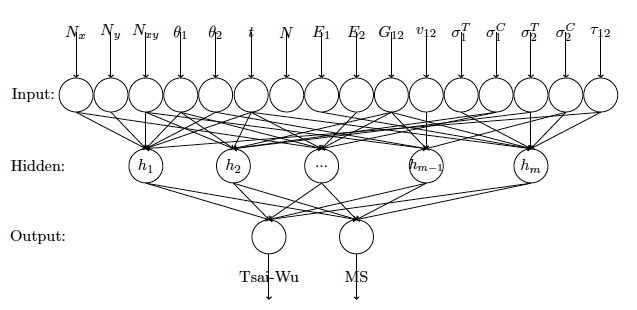
\includegraphics[width=0.9\textwidth]{./a0_figure_ann_for_clt_architecture.png}
\end{figure}
\subsection{Search Strategy}


The classic approach has always adopted binary strings to encode an alternative solutions. 


Tab.\ref{tab:parents1}  gives an example of the binary representation of an ANN
whose architecture is as shown in Fig.\ref{fig:parents1}. Each number in the
digit denotes the connection relationship between input and nodes in hidden
layer. It an connection exists, it's indicated by number one, otherwise, the
number takes zero. The first sixteen digits denotes the connection relationship, and the
last two digits are stand for  the corresponding kernal function. 

First,  random initialize ANN population, partial training every ANN, 
For the evolution of the topology,

\subsection{Performance estimation}
\cite{baker2017accelerating}








